\begin{figure}%[hbt!]
  \centering
  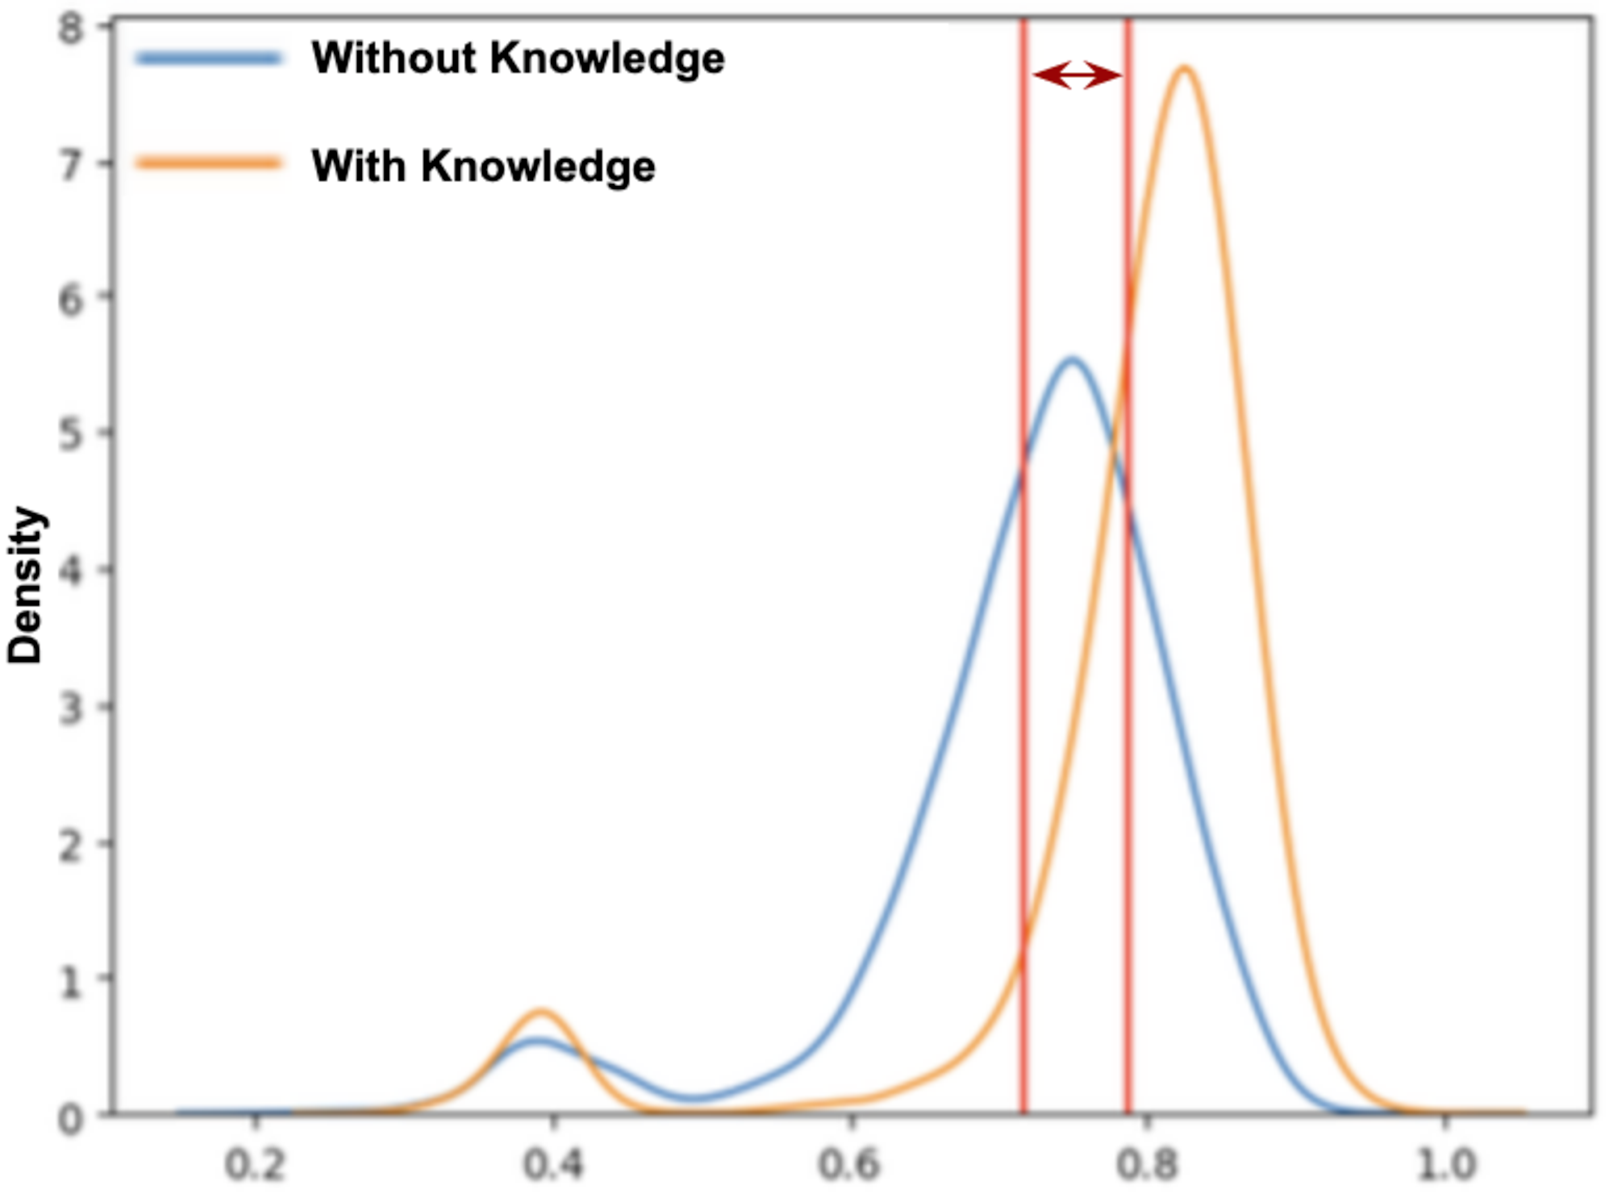
\includegraphics[width=7.8cm]{Figures/density-plot.pdf}
\vspace{-1em}
\caption{Density Plot demonstrates the difference between the similarities (cosine) of the image and text embeddings with and without knowledge. The inclusion of knowledge in the input gets text and image modalities closer by about 9.9\%.}
\vspace{-2em}
\label{fig:density-plot}
\end{figure} 


%As discussed earlier, we argue that contextual congruence is likely to be significant to capture semantic relationships in learning of multimodal representations. 
We examine the importance of contextual congruence by exploring the semantic distance between text and image modalities, and whether utilizing external knowledge from ConceptNet will get this distance closer and better reflect their semantics as explained below. 


\begin{figure*}[hbt!]
 % \vspace{-4em}
    \centering
  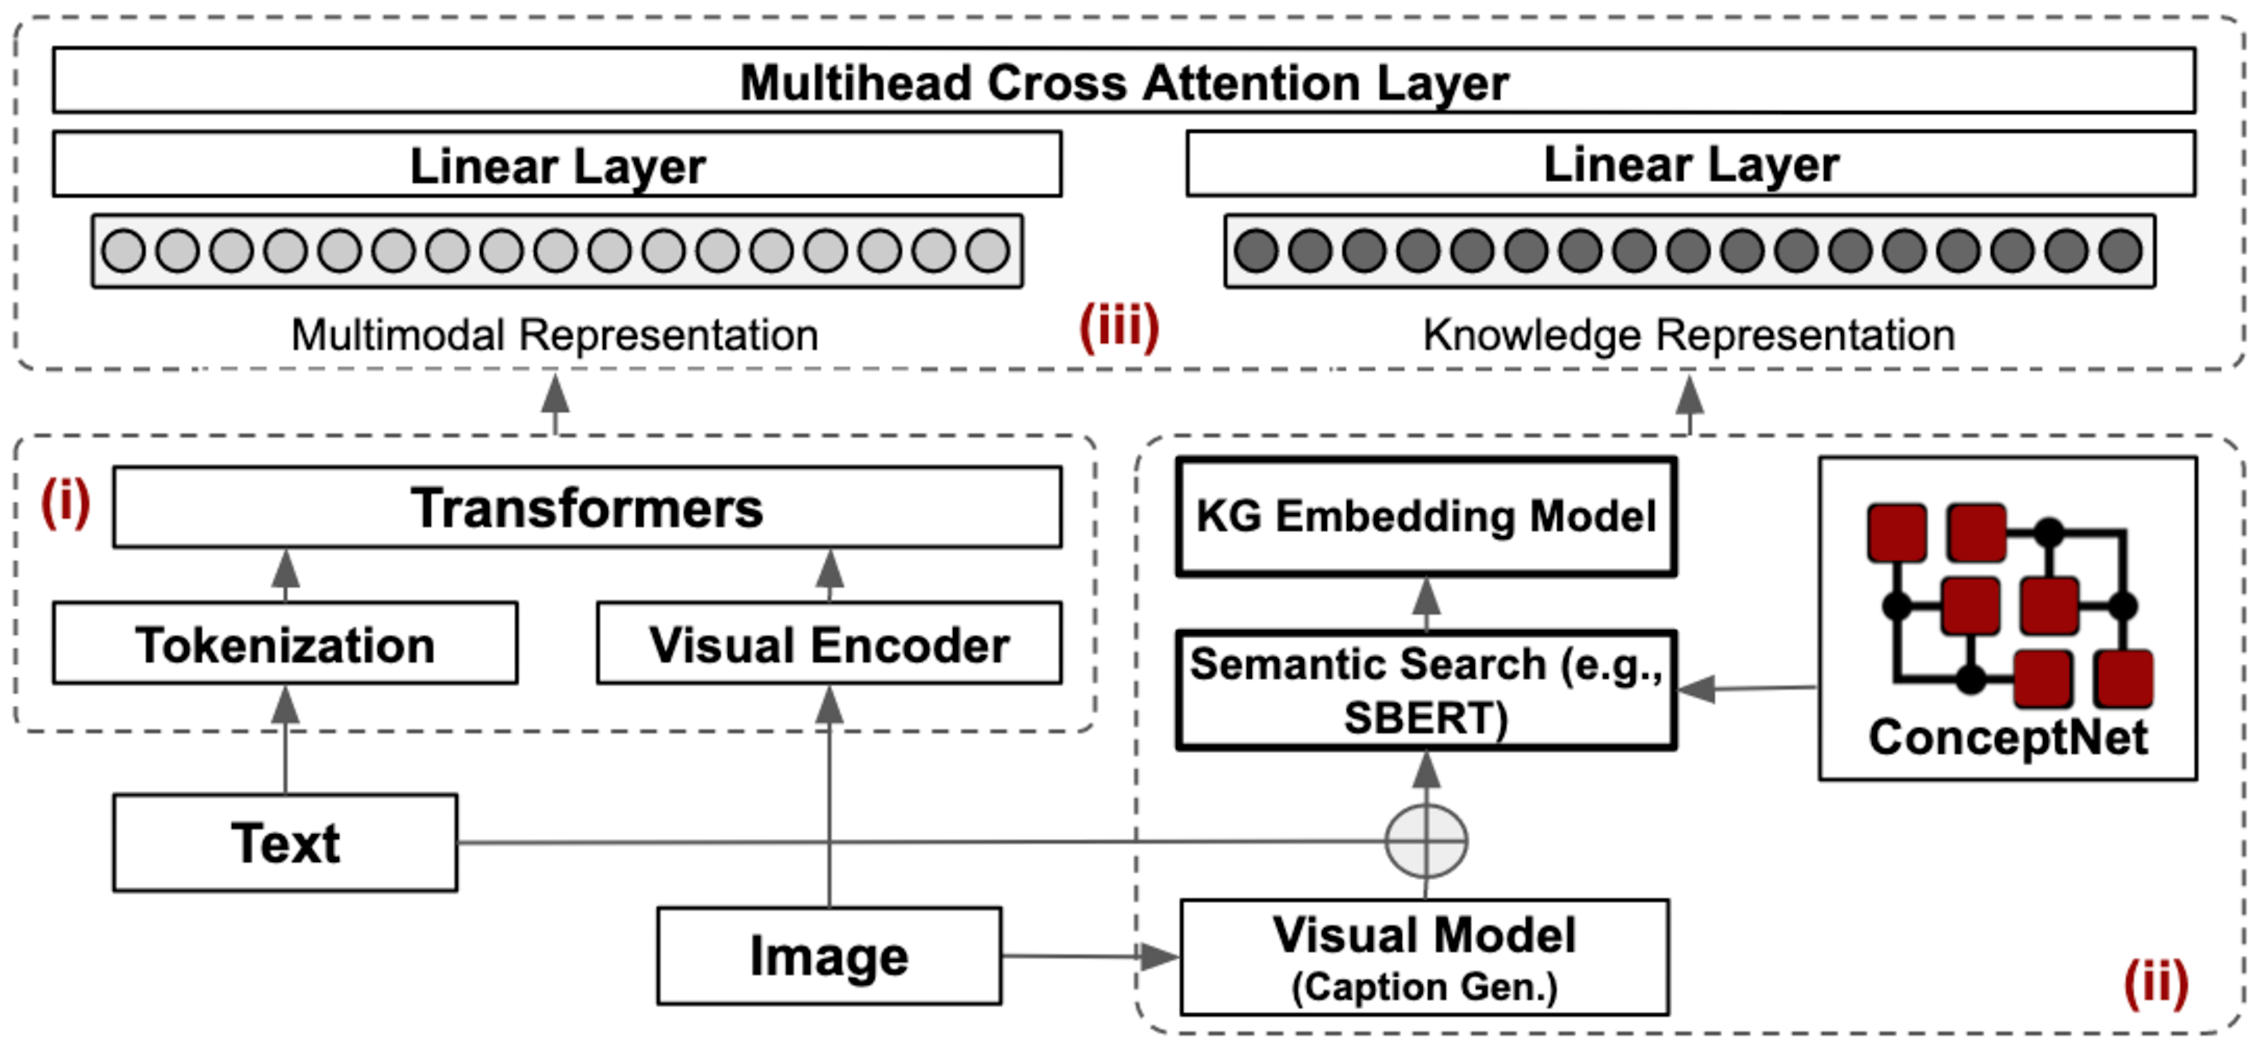
\includegraphics[width=17cm]{Figures/diagram.pdf}
\vspace{-0.8em}
\caption{Our approach consists of three main components: (i) multimodal learning, (ii) knowledge retrieval and representation, and (iii) Knowledge Fusion Layer. The Retrieval component identifies the most relevant concepts from ConceptNet. The concepts' KG embeddings are generated. The knowledge fusion layer fuses the multimodal representations with knowledge embeddings followed by Softmax.}
\vspace{-1em}
\label{fig:architecture}  
\end{figure*}

To demonstrate this idea, we generated the captions for image modality using BLIP, resulting in a textual description for each modality as text. For both text and image captions, we utilized semantic search (see Section Knowledge Retrieval) to extract the most relevant concepts. Then we simply appended these concepts to the input, which is a pair of text and image captions, to generate representations using BERT. We performed clustering analysis using DB-SCAN over the text and image captions ---we validated that the clusters represented text and image modalities.--- Our goal here is to show how the centroids of each cluster change when external knowledge is included in the input. Hence, we ran two clustering algorithms, with and without external knowledge.

Figure \ref{fig:embds-cluster} shows t-SNE visualizations of the text and image clusters created with and without external knowledge. The upper clusters (without knowledge) are more scattered whereas the lower clusters are denser. The centroids in the clusters with knowledge are also closer to each other, demonstrating the semantic distance is reduced because it can better reflect their semantic relationships. We ran the same experiment with different sizes of data points; 
%and our observation did not change as 
the clusters consistently got denser and centroids closer (see Figure \ref{fig:context_congruence_across_data_size} in the Appendix).
For each text-image pair in these clusters, we also measured semantic similarity using cosine and created their density plots (see Figure \ref{fig:density-plot}). 
%In other words, rather than measuring the semantic distance between centroids, we measured the similarity between image and text modalities in a pair. From figure 
Figure \ref{fig:density-plot} shows
%we can also observe that 
that the similarity between text and image modalities increased by about 9.9\%.

% To form contextual connections between the modalities, earlier efforts explored methods of combining the retrieved information from text and image, creating a new unique meaning, also called meaning multiplication \cite{bateman2014text,marsh2003taxonomy,zhang2018equal}. The example image in Figure \ref{fig:example-image} shows two women together with a hand gesture representing a "rock and roll" sign. The actual text caption provides information about a social movement without referral to anyone. When  the pair of image and text is considered together, the meaning can be clarified further as this is a campaign for women’s rights social movement where the two confident women represent the movement., Machines require to capture semantic relationships between the modalities to make the true semantic meaning of multimodal content \cite{rodd2012learning}, similar to humans. The multimodal LVMs \cite{brown2020language,li2023blip,liu2023visual} generates a caption for an only-image input explaining what is literally in the image with frequent hallucinations (see Table \ref{tab:generated-captions}). 


In addition, as we pair image and text modalities (see Figure \ref{fig:image-womens-movement-patriachy}),
% with the 
%human-generated 
% caption, 
the VLMs recognize relationships between modalities. %capturing the meaning to an extent while 
However, hallucinations are amplified by making non-existent connections and nonfactual information. Explicit knowledge from KGs can facilitate 
%the contextualizing and 
factual grounding.
%to capture the true meaning. 
We queried the KG to extract relevant concepts and simply include these with the pair of images and text as input for the VLMs such as Llava and BLIP. 
%We observe that the hallucinations are mitigated. 
This mitigates hallucinations. 
%For instance, in our example in 
As shown in Table \ref{tab:generated-caption-two-women}, the generated caption with knowledge does not include hallucination while containing contextual relationships from both the image and human caption.
%and is more contextually meaningful as the image and human caption are embedded in the meaning. The reader may find more 
Other examples appear in the appendix with generated captions (see Table \ref{tab:generated-captions}). 
These observations demonstrate the potential contribution of external knowledge to create more congruent multimodal representations by forming contextual relationships between modalities.  



